\documentclass{beamer}
\usepackage[T1]{fontenc} \usepackage{lmodern} \usepackage[utf8]{inputenc}
\usepackage[english]{babel} \usepackage{booktabs}
\usepackage{graphicx,subcaption} \usepackage{amssymb,amsmath}
\graphicspath{{../practical_info/}}
\usepackage[citestyle=authoryear,bibstyle=authoryear,backend=biber,url=false,doi=false,isbn=false]{biblatex} \bibliography{refs}
\usepackage{hyperref}

% Make Adobe Reader use the RGB rendering model for pages with transparency.
\pdfpageattr{/Group << /S /Transparency /I true /CS /DeviceRGB>>}

\mode<presentation>{
	\usetheme{Malmoe}
	\usecolortheme{beaver}
	\setbeamertemplate{footline}[page number]
	\setbeamertemplate{navigation symbols}{}
}

%------------------------------------------------

\newcommand{\todo}[1]{{\color{red} #1}}
\newcommand{\define}[1]{\item{\usebeamercolor[fg]{enumerate item}#1}:}
\newcommand{\HRule}{{\usebeamercolor[bg]{subsection in head/foot} \rule{\linewidth}{0.5mm}}}

%------------------------------------------------

\begin{document}

\begin{frame}[plain]
	\begin{center}

		\textsc{\large A Network Tour of Data Science (NTDS)}\\
		\vspace{0.7cm}

		\HRule
		\vspace{0.65cm}
		{
			\usebeamercolor[fg]{frametitle}
			%\textsc{\Large Practical Informations}\\
			\textsc{\Large Projects}\\
			%\textsc{\Large Laboratories}\\
			\vspace{0.4cm}
		}
		\HRule
		\vspace{1.0cm}

		\hspace{0.5cm}
		\begin{minipage}{0.4\linewidth}
			\footnotesize
			\textbf{Teachers} \\
			Pierre \textsc{Vandergheynst} \\
			Pascal \textsc{Frossard} \\
		\end{minipage}
		\begin{minipage}{0.4\linewidth}
			\footnotesize
			\textbf{Assistants} \\
			Michaël \textsc{Defferrard} \\
			Effrosyni \textsc{Simou} \\
			Hermina \textsc{Petric Maretić} \\
		\end{minipage}

		\vspace{0.7cm}
		\footnotesize EPFL LTS2 \& LTS4 laboratories\\
		\vspace{0.3cm}
		\footnotesize November 13, 2017

	\end{center}
\end{frame}

%------------------------------------------------

\begin{frame}
	\frametitle{Data Scientist}
	\begin{figure}
		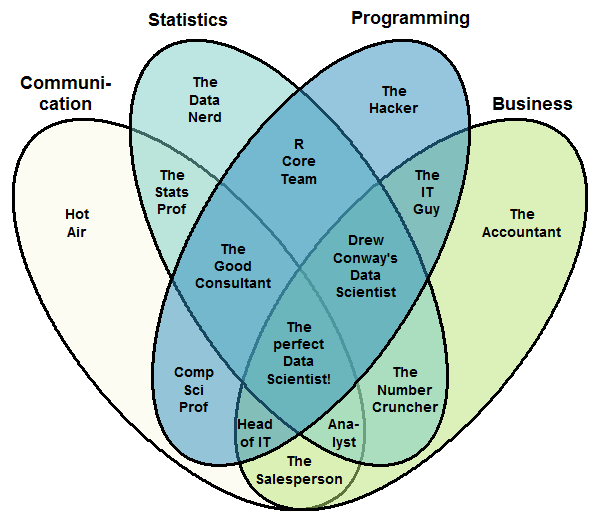
\includegraphics[height=0.8\textheight]{data_scientist}
	\end{figure}
\end{frame}

%------------------------------------------------

\begin{frame}
	\frametitle{Project}
	\begin{enumerate}
		\item Define a problem.
			\begin{itemize}
				\item Form groups of 3 or 4 students (4 preferred).
				\item Write a short but convincing proposal.
			\end{itemize}
		\vfill
		\item Solve it.
			\begin{itemize}
				\item Use the concepts learned in class.
				\item Follow the Data Science process.
			\end{itemize}
		\vfill
		\item Handle your solution for grading.
			\begin{itemize}
				\item Jupyter notebook as report.
				\item Oral presentation.
			\end{itemize}
	\end{enumerate}
\end{frame}

%------------------------------------------------

\begin{frame}
	\frametitle{Problem}
	\begin{center}
		Find a problem you want to solve. \\
		Think about your interests: scientific, hobbies, or otherwise.
	\end{center}
	\vfill
	%Sources of inspiration:
	Use \textbf{graphs} (A Network Tour) and \textbf{real data} (of Data Science).
	\vfill
	\begin{itemize}
		\define{Network Science} study networks! Tasks: analysis of properties, generative models, epidemics, etc.
		\define{Spectral Graph Theory} use the eigendecomposition of the graph Laplacian! Tasks: study of network properties, clustering, visualization, etc.
		\define{Graph Signal Processing} analyze signals defined on graphs! Tasks: information diffusion (e.g., for matrix completion and recommendation), denoising, semi-supervized learning, etc.\footnote{You can take a look at the \href{https://pygsp.readthedocs.io/en/stable/tutorials/index.html}{PyGSP tutorials.}}
	\end{itemize}
\end{frame}

%------------------------------------------------

\begin{frame}
	\frametitle{Data}
	\begin{itemize}
		\small
		\item Your own data, e.g., from your research.
		\vfill
		\item Call a web API or scrap a website (as assignments 1 and 3).
			Social websites are a wealth of information.\footnote{
			Twitter, Facebook, GitHub, Pinterest, Stack Overflow,
			YouTube, LinkedIn, Instagram, Tumblr, last.fm, reddit, etc.}
		\vfill
		\item From challenges, e.g., on \href{https://www.kaggle.com/}{kaggle} or \href{https://www.crowdai.org/}{crowdAI}.
		\vfill
		\item Some (list of) datasets.
			\begin{itemize}
				\scriptsize
				\item \href{https://github.com/mdeff/fma}{Free Music Archive (FMA)}.
				\item \href{https://doi.org/10.5281/zenodo.886484}{Wikipedia graph \& visits}. See e.g., \href{http://blog.miz.space/research/2017/08/14/wikipedia-collective-memory-dynamic-graph-analysis-graphx-spark-scala-time-series-network/}{this blog post}.
				\item \href{http://snap.stanford.edu/data/index.html}{Stanford Large Network Dataset Collection (SNAP)}.
				\item \href{https://linqs.soe.ucsc.edu/node/236}{Citation networks (Cora, arXiv, PubMed)}. See e.g., \href{http://paperscape.org/}{arXiv viz}.
				\item The \href{http://networkrepository.com}{Network Repository}.
				\item \href{https://github.com/briatte/awesome-network-analysis\#datasets}{A list of datasets for network analysis}.
				\item \href{https://github.com/caesar0301/awesome-public-datasets}{Awesome Public Datasets}.
				\item \href{https://opendata.swiss/en/}{Swiss open data}.
			\end{itemize}
		\vfill
		\item More: transportation, communication, neural (artificial or biological), energy networks.
		\item Any other. Discuss with us!
	\end{itemize}
\end{frame}

%------------------------------------------------

\begin{frame}
	\frametitle{Data Science Process}
	\begin{figure}
		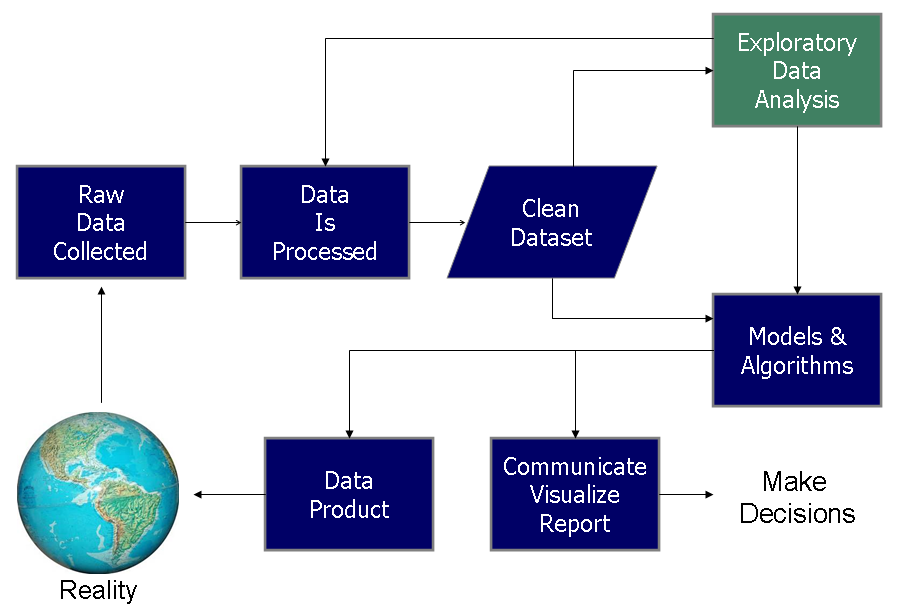
\includegraphics[width=\textwidth]{data_science_process}
	\end{figure}
\end{frame}

%------------------------------------------------

\begin{frame}
	\frametitle{Structure}
	The structure of the notebook shall follow the Data Science process seen
	during the lab sessions.
	\vfill
	\begin{enumerate}
		\define{Data acquisition} from the web, a database, a flat file, etc.
			This includes cleaning the data.
		\vfill
		\define{Data exploration} some exploratory analysis to describe
			properties of the data and understand the content.
		\vfill
		\define{Data exploitation} use the data to solve a task, to infer
			knowledge, to draw conclusions.
			The concepts or algorithms taught in class must be used.
		\vfill
		\define{Conclusion} discuss the results and summarize your findings.
			What did we learn from the data and the project?
	\end{enumerate}
\end{frame}

%------------------------------------------------

\begin{frame}
	\frametitle{Practical aspects}
	\begin{itemize}
		\item Please isolate code blocks in functions and put those in a
			separate Python module.
		%\item Maximize the use of external libraries. You should invest time
			%in the problem, not in reinventing the wheel.
		\vfill
		\item Your notebook should be clean and legible. They are akin to a report.
		\vfill
		\item You can take inspirations from the notebooks seen during the
			lab sessions.
		\vfill
		\item Look at \href{https://github.com/mdeff/ntds_2016\#projects}{last year projects}.
	\end{itemize}
\end{frame}

%------------------------------------------------

\begin{frame}
	\frametitle{Rules}
	\begin{itemize}
		\item The project includes graph and network data aspects, and more
			generally falls under the scope of the class.
		\vfill
		\item Form groups of 3 or 4 students. No less, no more.
			\begin{itemize}
				\item One member of the group uploads the deliverables.
				\item The names of all members should appear clearly.
			\end{itemize}
		\vfill
		\item The project can be shared with another course (e.g., data
			visualization or ADA). State it clearly and specify what gets
			graded for which course.
		\item The project should follow the data acquisition, exploration and
			exploitation workflow.
		\vfill
		\item Data must not be synthetic. While manually collecting data is
			optional, i.e., the use of datasets is allowed, it is a plus.
		\vfill
		\item Each member of a team shall contribute equally to the project.
	\end{itemize}
\end{frame}

%------------------------------------------------

\begin{frame}
	\frametitle{Organization}
	\begin{enumerate}
		\define{Proposal} define the problem and explain your plan.
			\begin{itemize}
				\item Single page document.
				\item Organize yourselves in groups of 3 or 4 students.
				\item Deadline: Tuesday, November 28, 2017. Upload on Moodle.
				\item Not graded. Discussion with TAs will follow.
			\end{itemize}
		\vfill
		\define{Report} your solution, using the theory seen in class and the
			practical skills trained during labs.
			\begin{itemize}
				\item Jupyter notebook with text, math, code, analysis and
					results.
				\item The notebook will be posted on the course git repository,
					on GitHub. You can use it for your portfolio!
				\item Deadline: Friday, January 12, 2017. Upload on Moodle.
				\item Graded (project accounts for 50\% of class grade).
			\end{itemize}
		\vfill
		\define{Presentation} impress us with your work!
			\begin{itemize}
				\item Presentation of 15 minutes followed by 5 minutes of questions.
				\item Each group member must talk.
				\item Register for January 24 or 25 (once exams are scheduled).
				\item Graded (project accounts for 50\% of class grade).
			\end{itemize}
	\end{enumerate}
\end{frame}

%------------------------------------------------

\begin{frame}
	\Huge
	\begin{center}
		\vspace{0.2cm}
		Have fun! \hspace{1cm} Questions?
		\vspace{0.5cm}
		\begin{figure}
		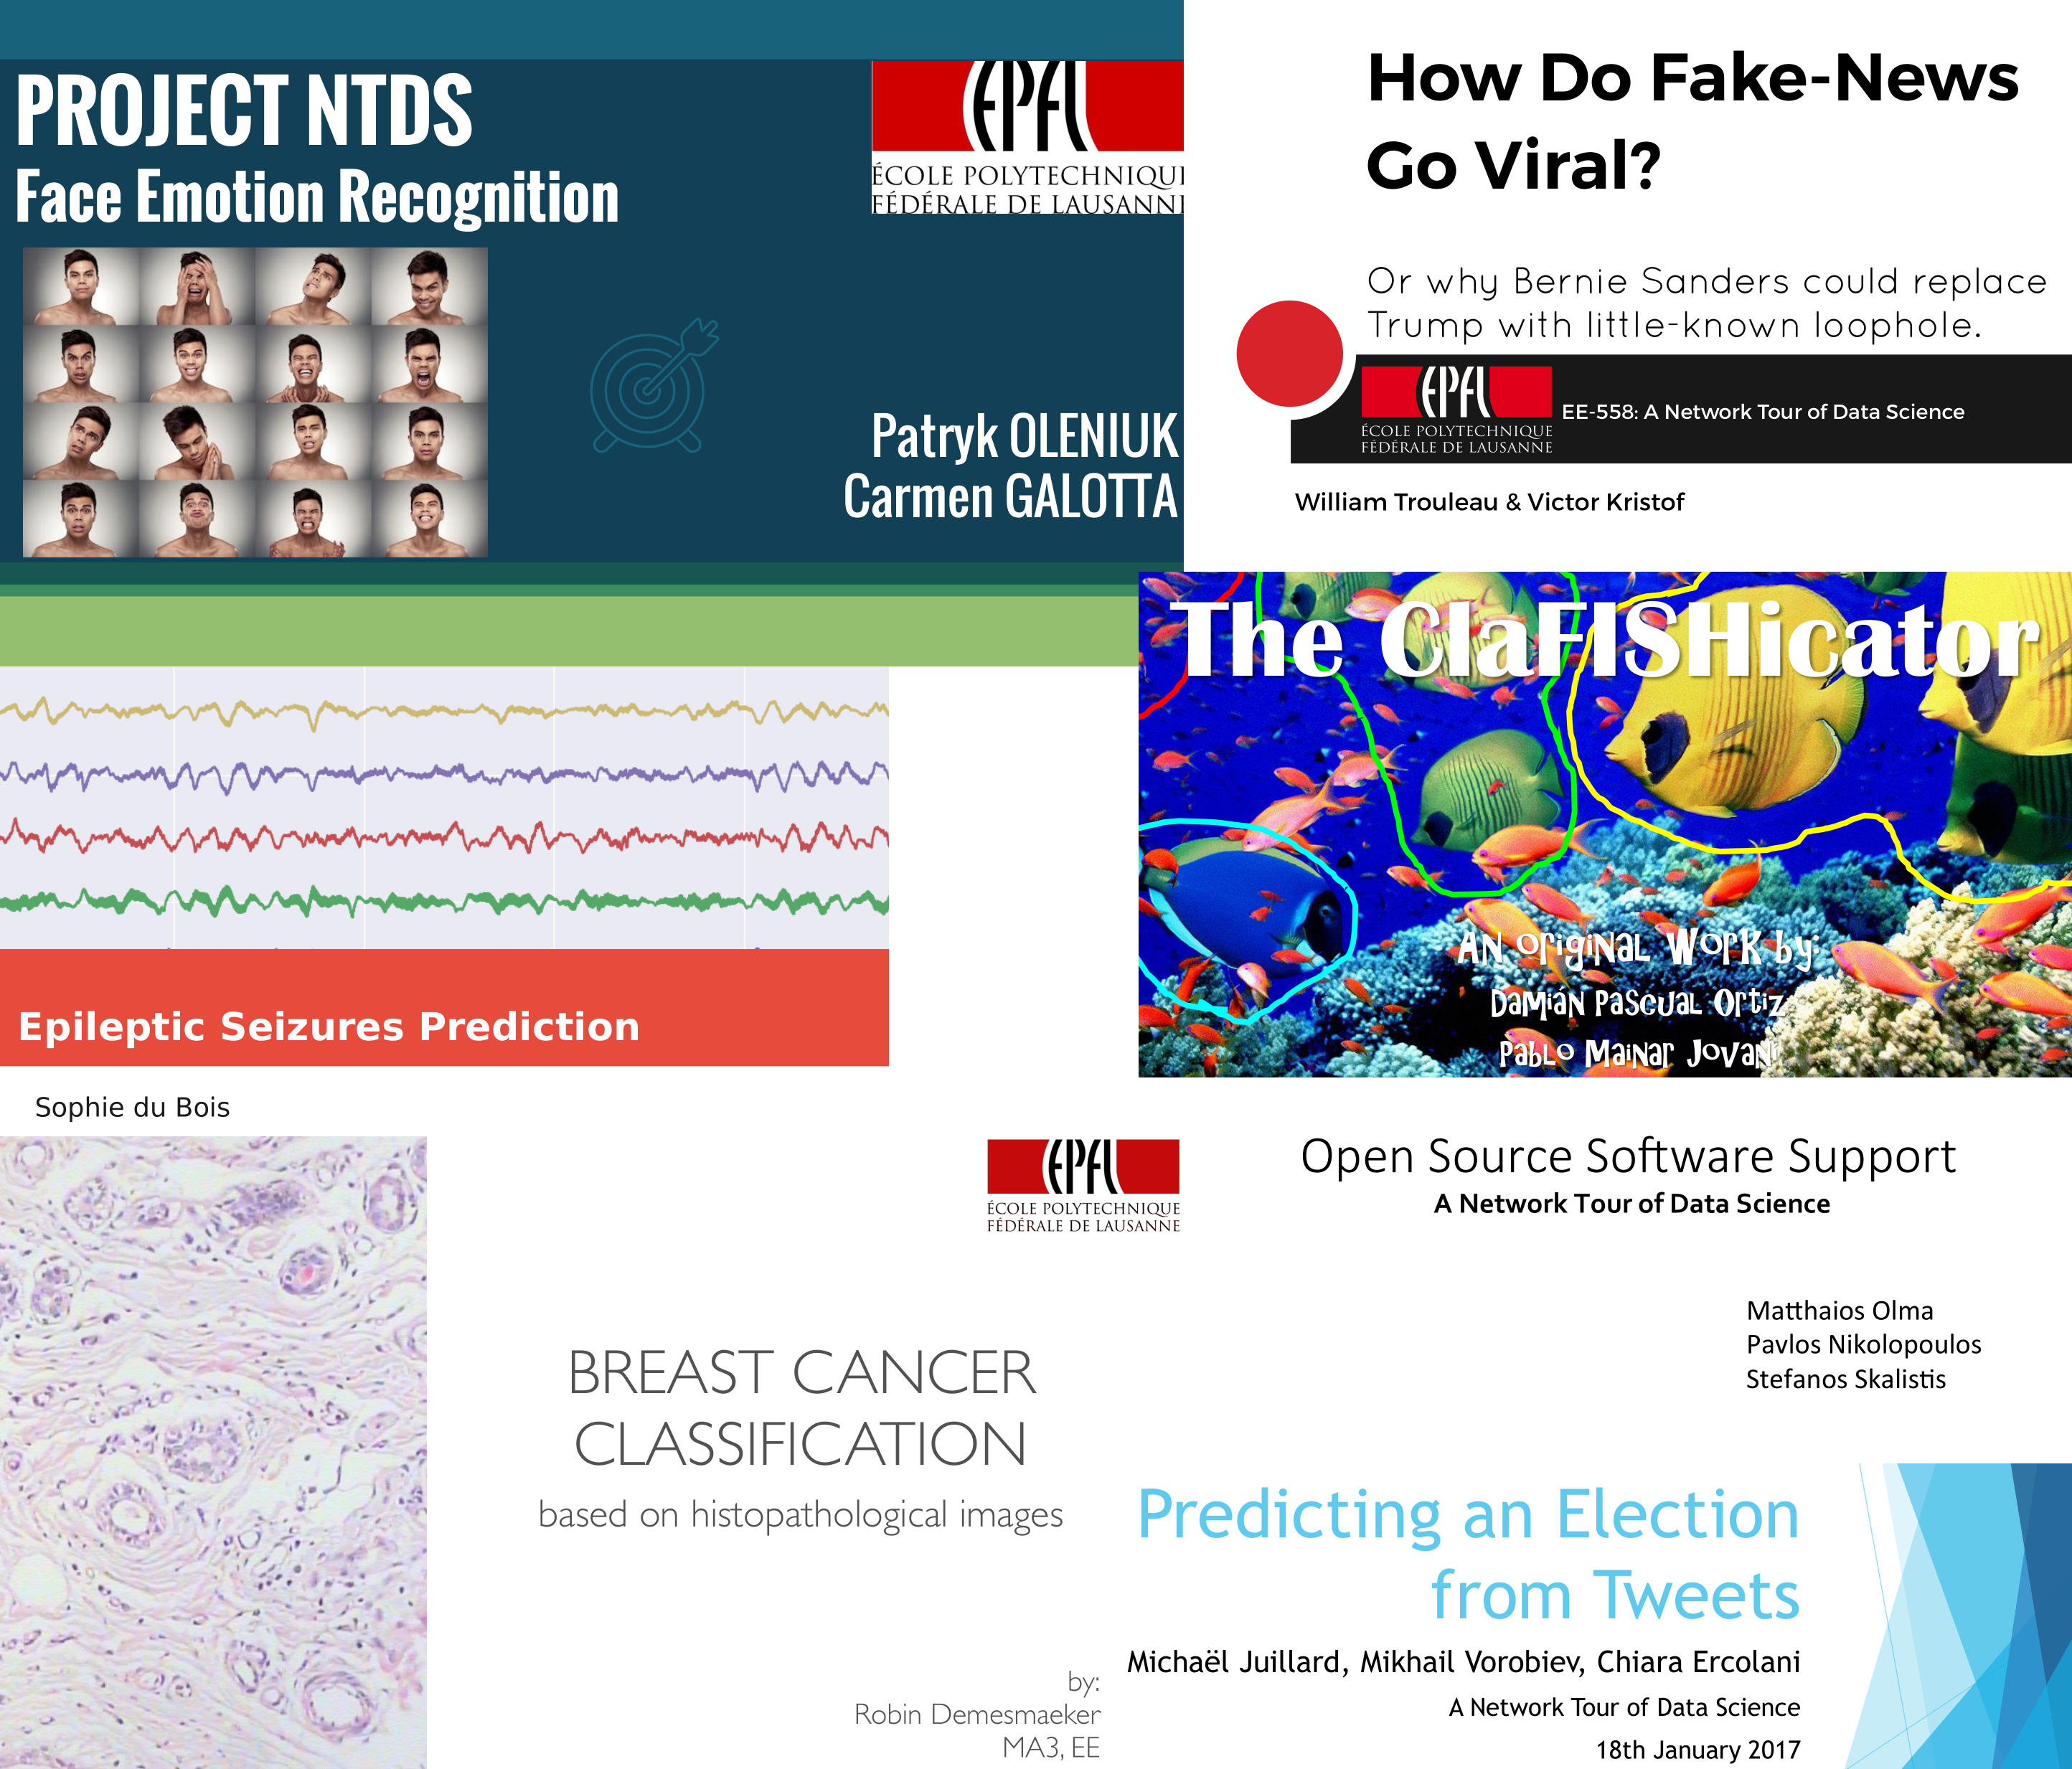
\includegraphics[width=\linewidth]{projects_2016}
		\end{figure}
	\end{center}
\end{frame}

\end{document}
